\documentclass[
%a4paper,12pt
encoding=utf8
]{../twoeskd}

% \usepackage{eskdappsheet}

% Packages required by doxygen
\usepackage[export]{adjustbox} % also loads graphicx
%\usepackage[utf8]{inputenc}
\usepackage{multicol}
\usepackage{multirow}
\usepackage{makeidx}
\usepackage{caption}
\usepackage{graphicx}

% NLS support packages
\usepackage[T2A]{fontenc}
\usepackage[russian]{babel}
\usepackage{pscyr}

% Font selection
\usepackage{courier}
\usepackage{amssymb}

% Page & text layout
% \usepackage{geometry}
% \geometry{%
%   a4paper,%
%   top=2.5cm,%
%   bottom=4.5cm,%
%   left=2.5cm,%
%   right=2.5cm%
% }
%\setlength{\emergencystretch}{15pt}
\setlength{\parindent}{0cm}
\setlength{\parskip}{0.2cm}

% Headers & footers
% \usepackage{fancyhdr}
% \pagestyle{fancyplain}
% \fancyhead[L]{\fancyplain{}{}}
% \fancyhead[C]{\fancyplain{}{\scriptsize\textbf{RU.17701729.509000 ТЗ 01-1-ЛУ}}}
% \fancyhead[R]{\fancyplain{}{}}
% \fancyfoot[L]{\fancyplain{}{}}
% \fancyfoot[C]{\fancyplain{}{}}
% \fancyfoot[R]{\fancyplain{}{}}

% debug to see the frame borders
% from https://en.wikibooks.org/wiki/LaTeX/Page_Layout
% \usepackage{showframe}

% Indices & bibliography
\usepackage{natbib}
\usepackage[titles]{tocloft}
\setcounter{tocdepth}{3}
\setcounter{secnumdepth}{5}

% change style of titles in \section{}
\usepackage{titlesec}
\titleformat{\section}[hang]{\huge\bfseries\center}{\thetitle.}{1em}{}
\titleformat{\subsection}[hang]{\Large\normalfont\raggedright}{\thetitle.}{1em}{\underline}
\titleformat{\subsubsection}[hang]{\large\normalfont\raggedright}{\thetitle.}{1pt}{}

% Packages for text layout in normal mode
% \usepackage[parfill]{parskip} % автоматом делает пустые линии между параграфами, там где они есть в тексте
% \usepackage{indentfirst} % indent even in first paragraph
\usepackage{setspace}	 % controls space between lines
\setstretch{1} % space between lines
\setlength\parindent{0.9cm} % size of indent for every paragraph
\usepackage{csquotes}% превратить " " в красивые двойные кавычки
\MakeOuterQuote{"}


% this makes items spacing single-spaced in enumerations.
\newenvironment{my_enumerate}{
\begin{enumerate}
  \setlength{\itemsep}{1pt}
  \setlength{\parskip}{0pt}
  \setlength{\parsep}{0pt}}{\end{enumerate}
}


% Custom commands
% configure eskd
\titleTop{
\textbf{\Large ПРАВИТЕЛЬСТВО РОССИЙСКОЙ ФЕДЕРАЦИИ \\
НАЦИОНАЛЬНЫЙ ИССЛЕДОВАТЕЛЬСКИЙ УНИВЕРСИТЕТ \\
«ВЫСШАЯ ШКОЛА ЭКОНОМИКИ» } \\
\vspace*{0.2cm}
{\small Факультет компьютерных наук \\
Департамент программнoй инженерии \\
}
}
\titleDesignedBy{Студент группы БПИ 151 НИУ ВШЭ}{Абрамов А.M.}
\titleAgreedBy{%
\parbox[t]{7cm} {
Профессор департамента \\
программной инженерии \\
факультета компьютерных наук \\
канд. техн. наук \\
}}{Гринкруг Е. М.}
\titleApprovedBy{
\parbox[t]{10cm} {
Академический руководитель \\
образовательной программы \\
«Программная инженерия» \\
профессор департамента программной \\
инженерии канд. техн. наук \\
}}{Шилов В. В.}
\titleName{ПРОГРАММАТОР МИКРОКОНТРОЛЛЕРОВ PIC НА ОСНОВЕ ORANGE PI LITE}
\workTypeId{RU.17701729.509000 51 01-1}

\titleSubname{Программа и методика испытаний}

% Custom packages
\usepackage{pdfpages}

\makeindex

%===== C O N T E N T S =====


\begin{document}
% Titlepage & ToC
\pagenumbering{roman}

% some water filling text, that is pointless but adds text
% \input{annotation}

\newpage
\pagenumbering{arabic}
\tableofcontents
% \pagenumbering{arabic}

% --- add my custom headers ---
\newpage
\section{Объект испытаний}
\subsection{Наименование}
Наименование: «Программатор микроконтроллеров PIC на основе Orange PI Lite». \\
Наименование на английском: «Programmer for PIC Microcontrollers Based on Orange PI Lite». \\

\subsection{Область применения}
Программа и электронная схема предназначена для работы на тонком кленте Orange Pi Lite с операционной системой семейства Linux. Программа и схема могут использоваться в учебных целях для демонстации основных компонентов необходимых для прошивки микроконтроллера. Они предоставляют новое направление использования тонкого клиента Orange Pi Lite. Ими может воспользоваться любой человек, желающий запрограммировать микроконтроллер, не имеющий на руках официального программатора, но у которого есть Orange Pi Lite. Данная программа и электронаня схема могут использоваться в качестве дешевой, простой и быстрой алтернативы к покупке официального программатора.


\newpage
\section{Цель испытаний}
Цель проведения испытаний, - проверить, что разработанная программа соответствует требованиям к функциональности и надежности, изложенным в техническом задании к программе.


\newpage
\section{Требования к програмному изделию}


%=========================================
\subsection{Требования к функциональным характеристикам}
\subsubsection{Требования к составу выполняемых функций}
\begin{my_enumerate}
\item Чтение данных из формата INTEL HEX8M для хранения программы прошивки.
\item Возможность отдельной записи EEPROM памяти, не стирая програмную память микроконтроллера.
\item Поддержка 3 линеек микроконтроллеров серии 16F: 627A / 628A / 648A.
\item Проверка входного файла на корректность.
\item Графический интерфейс для оперирования программой.
\item Интерфейс командной строки для оперирования программой.
\item Повышаюший переходник с 3.3В на 5В для взаимодействия с микроконтроллером.
\item Схемотехника для платы которая позволяет подключить микроконтроллер к тонкому клиенту Orange Pi Lite.
\item Завершенные, работающие схемы на макетной плате.
\item Схемы разводки макетной платы для подключения микроконтроллера к Orange Pi Lite. 
\end{my_enumerate}

\subsubsection{Требования к организации входных и выходных данных}
Входными данными для работы программатора являются скомпилированный файл программы, микроконтроллер подключенный к плате, а также (для обеспечения взаимодействия с пользователем) клавиатура и/или мышь. Входной файл данных может быть созданн в любой среде разработки и любым компилятором поддершивающим формат INTEL HEX8M. Примером такой среды разработки является MPLAB X (https://www.microchip.com/, разработчик: коммерческая организация Microchip Ltd.).

\begin{my_enumerate}
\item Из-за огромного количества серий микроконтроллеров поддерживать их все не представляется возможным. Поэтому программа должна работать только с микроконтроллерами PIC серии 16F, конкретно с линейками 627A / 628A / 648A.
\item Файл программы должен соответствовать формату INTEL HEX8M. По сравнению с двумя другими часто встречающимися форматами INTEL HEX8S, INTEL HEХ32, данный формат наиболее оптимально подходит под серию 16F. В силу того что память 14-битных микроконтроллеров не превышает 64 килобайт (здесь подходит формат HEX32) и програмное слово не нуждаеться в разбиении на высокий и низкий байт как в 16-битных микроконтроллерах (здесь подходит формат HEX8S).
\item Пользователь должен иметь возможность модифицировать следующие входные данные в процессе работы программы в усливиях графического интерфейса и перед запуском программы в командной строке:
\begin{my_enumerate}
\item Указать что требуется запись EEPROM памети без модификации програмной памяти микроконтроллера.
\item Указать что требуется проверить входной файл на ошибки.
\item Указать что требуется записать входной файл в програмную память и в EEPROM память микроконтроллера.
\item Поменять уровень колличества сообщений выводимих программой пользователю.
\item Отменить процесс программирования.
\end{my_enumerate}
\end{my_enumerate}

\medskip
Выходными данными для программатора является запрограммированный микроконтроллер, данные на экране и индикатор программирования на плате программатора.


\subsubsection{Прочие требования}
\begin{enumerate}
\item Поддержка изменения размеров окна.
\item Использование Qt для создания интерфейса.
\end{enumerate}

%=========================================
\subsection{Требования к временным характеристикам}
\begin{enumerate}
\item Задержка между сигналом к началом программирования не должна быть меньше чем 0.001 секунда и не должна превышать 0.1 секунд для файлов программ размером меньше чем 5 килобайт.
\end{enumerate}


%=========================================
\subsection{Требования к интерфейсу}
Интерфейс должен быть прост в использовании. Он должен предоставлять возможность
\begin{my_enumerate}
\item Прочитать данные из формата INTEL HEX8M для хранения программы прошивки.
\item Возможность запрограммировать EEPROM память, не стирая програмную память микроконтроллера.
\item Проверить входной файл на корректность.
\end{my_enumerate}

Командный интерфейс должен предоставлять те же возможности что и графический интерфейс и следовать стандартам принятым при создании интерфейсом командной строки в системе Linux.

%=========================================
\subsection{Требования к надежности}
\subsubsection{Обеспечение устойчивого функционирования программы}
Программа не должна вне зависимости от входных данных или действий оператора завершатся аварийно. При некорректно введенных параметрах пользователю должно отображаться сообщение об ошибке.
\subsubsection{Время восстановления после отказа}
Требования к восстановлению после отказа не предъявляются.
\subsubsection{Отказы из-за некорректных действий оператора}
В случае открытия файла, не соответствующему требованиям ко входным данным, пользователю должно отображаться сообщение об ошибке.


\newpage
\section{Требования к програмной документации}
\subsection{Предварительный состав программной документации}
В обязательном порядке должны входить:
\begin{my_enumerate}
\item Техническое задание  (ГОСТ 19.201-78)
\item Пояснительная записка  (ГОСТ 19.404-79)
\item Руководство оператора  (ГОСТ 19.505-79)
\item Программа и методика испытаний (ГОСТ 19.301-79*)
\item Текст программы  (ГОСТ 19.401-78*)
\end{my_enumerate}



\newpage
\section{Средства и порядок испытаний}
%=========================================
\subsection{Параметры технических средств, используемых во время испытаний}
Для оптимальной работы приложения необходимо учесть следующие системные требования:
\begin{my_enumerate}
\item Тонкий клиент Orange Pi Lite, оснащенный:
    \begin{my_enumerate}
    \item Обязательно процессор Allwinner H3 с тактовой частотой 1 гигагерц (ГГц) или выше;
    \item 0.5 ГБ оперативной памяти (ОЗУ);
    \item 0.5 ГБ свободного места на жестком диске;
    \item Периферия: выход GPIO типа Rasberry Pi B+
    \end{my_enumerate}
\item Опционально: Компьютер для удаленного доступа к Orange Pi Lite, оснащенный:
    \begin{my_enumerate}
    \item Обязательно 64-разрядный (x64) процессор с тактовой частотой 1 гигагерц (ГГц) или выше;
    \item 1 ГБ оперативной памяти (ОЗУ);
    \item 1.5 ГБ свободного места на жестком диске;
    \item Wifi модулем (если Orange Pi Lite подключен к сети, то можно воспользоваться и стандартным Ethernet портом) или TTL переходником для подключения к тонкому клиенту Orange Pi Lite.
    \end{my_enumerate}
\item Монитор
\item Мышь
\item Клавиатура
\end{my_enumerate}


%=========================================
\subsection{Программные средства, необходимые для проведения испытаний}
Исходный код программы для контролирования программатора обязательно должен быть написан с использованием языка C. Приложению необходим тонкий клиент с операционной системой производной от Debian с версией ядра не ниже 3.1. Приложение можно запускать как с  самого Orange Pi Lite, так и с компьютера имеющего удаленный доступ к Orange Pi Lite. В данном случае на удаленном компьютере и на тонком клиенте должны быть установленны программы для настроек удаленного доступа (например SSH, VNC viewer, TTY serial console). Для данных програм подходит любой дистрибутив Linux или 64-битная операционная система Windows 7 или более поздняя версия Windows.


%=========================================
\subsection{Порядок проведения испытаний}
Испытания должны проводиться в следующем порядке:
\begin{my_enumerate}
\item Проверка требований к документации.
\item Проверка требований к интерфейсу.
\item Проверка требований к функциональным возможностям программы.
\item Проверка требований надежности.
\end{my_enumerate}


%=========================================
\subsection{Условия проведения испытаний}

\subsubsection{Требования к численности и калификации персонала}
Минимальное количество персонала, требуемого для работы программы: 1 оператор. Пользователь программы должен иметь образование не ниже среднего, обладать практическими навыками работы с компьютером и электронникой.




\newpage
\section{Методы испытаний}
Испытания представляют собой процесс установления соответствия программы и
программной документации заданным требованиям.

\subsubsection{Проверка требований к документации}
Проверяеться наличие всех документов перечисленных в пyнкте 4.1 данного документа и их соответствие ГОСТ.

\subsection{Проверка требований к интерфейсу}
Интерфейс соответствует схеме, указанной в техническом задании.

\begin{figure}[h!]
    \centering
    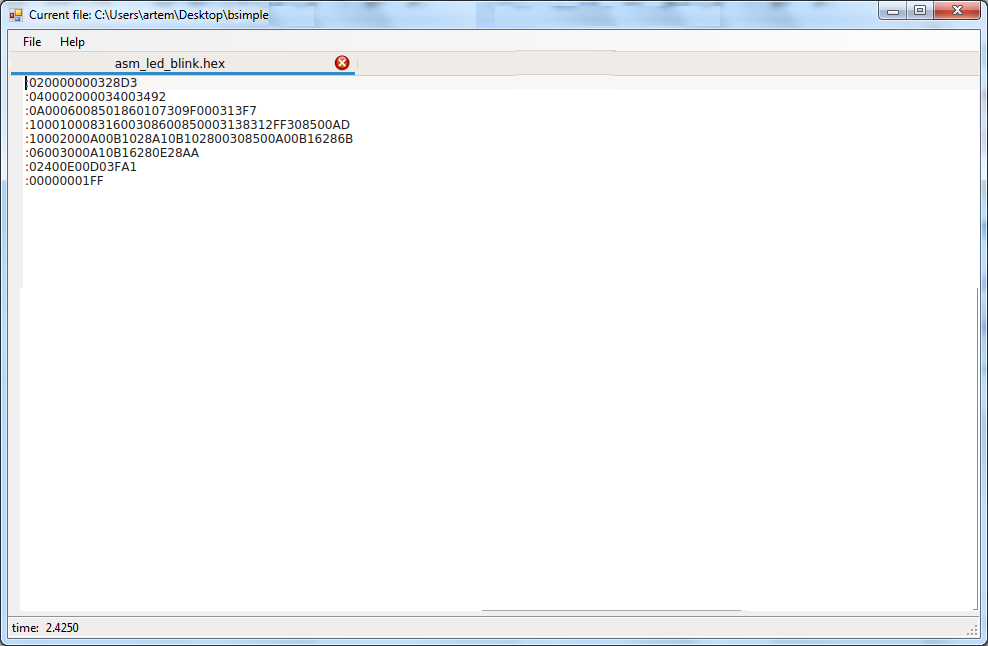
\includegraphics[width=0.5\textwidth]{../screenshots/interface_map.png}
    \caption{Изображение интерфейса программы}
\end{figure}

Интерфейс командной строки также соответствует предъявленным требованиям.

\subsection{Проверка требований к функциональным характеристикам}
Для загрузки данных из формата INTEL HEX8M (.hex) необходимо выбрать его в меню "Open":

\begin{figure}[h!]
    \centering
    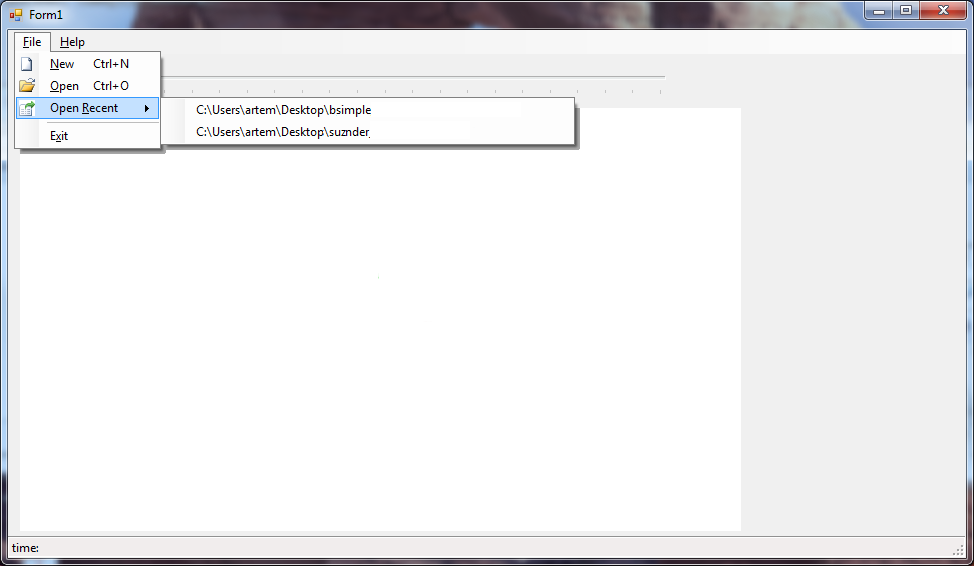
\includegraphics[width=0.8\textwidth]{../screenshots/file_menu_with_recent.png}
    \caption{Загрузка файла}
\end{figure}

Откроется диалог выбора файла:
\begin{figure}[h!]
    \centering
    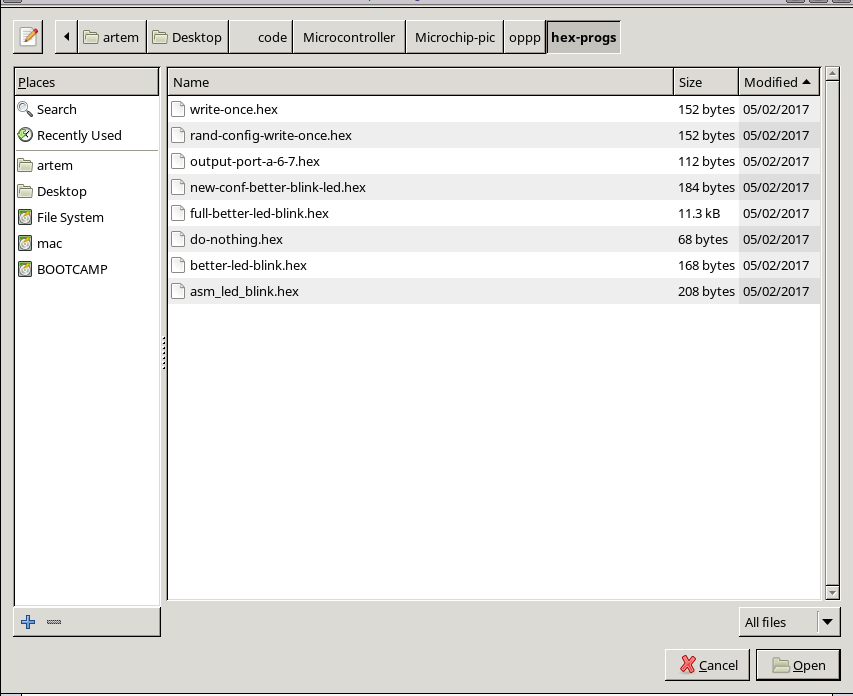
\includegraphics[width=0.5\textwidth]{../screenshots/open_file_dialog.png}
    \caption{Диалог выбора файла}
\end{figure}

После загрузки файла, его содержание будет отображенно в центральном окне.


%=================
Также есть панель для настоек работы программы позволяющая изменять следующие параметры:
\begin{my_enumerate}
\item Указать что требуется запись EEPROM памети без модификации програмной памяти микроконтроллера.
\item Указать что требуется проверить входной файл на ошибки.
\item Указать что требуется записать входной файл в програмную память и в EEPROM память микроконтроллера.
\item Поменять уровень колличества сообщений выводимих программой пользователю.
\item Отменить процесс программирования.
\end{my_enumerate}


%=================
Поддерживатся изменение размеров окна приложения.


\subsection{Проверка требований к надежности}
Оператор должен воспользоваться всеми функциями программы и убедиться, что они не приводят к ее аварийному завершению.


\newpage
\section{Приложение 1. Терминология}
\subsection{Терминология}
\begin{description}

\item[Корневая вершина (англ. root node)]  
Самый верхний узел дерева.

\item[Полигональная сетка (жарг. меш от англ. polygon mesh)]
Совокупность вершин, рёбер и граней, которые определяют форму многогранного объекта в трехмерной компьютерной графике и объёмном моделировании. Гранями являются треугольники.

\item[Дерево]
Связный ациклический граф. Связность означает наличие путей между любой парой вершин, ацикличность — отсутствие циклов и то, что между парами вершин имеется только по одному пути.

\item[Степень вершины]
Количество инцидентных ей (входящих/исходящих из нее) ребер.

\item[Интерполяция, интерполирование анимации]
Способ нахождения промежуточных значений состояния анимации по имеющемуся дискретному набору известных значений.

\item[Z-буферизация]
В компьютерной трёхмерной графике способ учёта удалённости элемента изображения. Представляет собой один из вариантов решения «проблемы видимости»

\item[Z-конфликт (англ. Z–fighting)]
Если два объекта имеют близкую Z-координату, иногда, в зависимости от точки обзора, показывается то один, то другой, то оба полосатым узором.

\item[OpenGL (Open Graphics Library)]
Спецификация, определяющая независимый от языка программирования платформонезависимый программный интерфейс для написания приложений, использующих двумерную и трёхмерную компьютерную графику. На платформе Windows конкурирует с Direct3D.

\item[Рендеринг (англ. rendering — «визуализация»)]
Термин в компьютерной графике, обозначающий процесс получения изображения по модели с помощью компьютерной программы.

\item[Текстура]
Растровое изображение, накладываемое на поверхность полигональной модели для придания ей цвета, окраски или иллюзии рельефа. Приблизительно использование текстур можно легко представить как рисунок на поверхности скульптурного изображения.

\end{description}



%\newpage
%\section{Приложение 2. Схема интерфейса программы}
%\begin{figure}[h!]
    \centering
    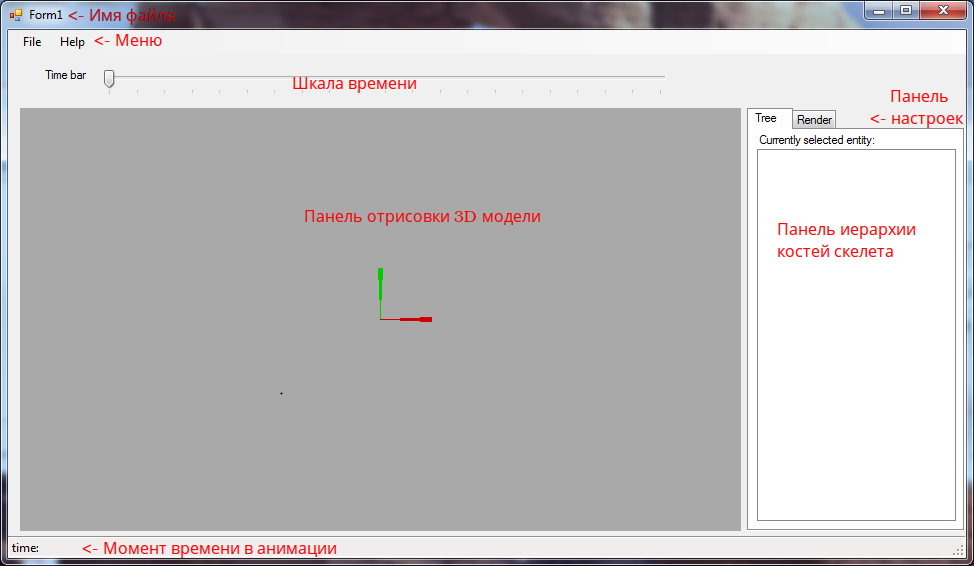
\includegraphics[width=0.8\textwidth]{../screenshots/main_empty.png}
    \caption{Схема интерфейса}
\end{figure}


\newpage
\section{Приложение 2. Список используемой литературы}
\subsection{Список используемой литературы}
\begin{my_enumerate}
\item
ГОСТ 19.101-77 Виды программ и программных документов
//Единая система программной документации. -М.: ИПК Издательство стандартов, 2.: 001.

\item
ГОСТ 19.103-77 Обозначения программ и программных документов. //Единая система программной документации. -М.: ИПК Издательство стандартов, 2001.

\item
ГОСТ 19.104-78 Основные надписи //Единая система программной документации. -М.: ИПК Издательство стандартов, 2001.

\item 
ГОСТ 19.105-78 Общие требования к программным документам. //Единая система
программной документации. – М.: ИПК Издательство стандартов, 2001.

\end{my_enumerate}




% Index
\newpage
\eskdListOfChanges

% \phantomsection
% \addcontentsline{toc}{section}{Алфавитный указатель}
% \printindex

\end{document}
